\documentclass[a4paper]{article}
\usepackage[spanish]{babel}
\usepackage[utf8]{inputenc}
\usepackage{fancyhdr}
\usepackage{verbatim}
\usepackage{charter} % tipografia
%\usepackage{graphicx}
\usepackage[pdftex]{graphicx}
\usepackage{bm} % bold font in math mode
\usepackage{sidecap}
\usepackage{caption}
\usepackage{subcaption}
\usepackage{booktabs}
\usepackage{makeidx}
\usepackage{float}
\usepackage{amsmath, amsthm, amssymb}
\newtheorem{theorem}{Teorema}
\newtheorem{customthm}{Teorema}
\newtheorem{corollary}{Corolario}[theorem]
\newtheorem{proposition}[theorem]{Proposición}
\newtheorem{innercustomlemma}{Lemma}
\newenvironment{customlemma}[1]
  {\renewcommand\theinnercustomlemma{#1}\innercustomlemma}
  {\endinnercustomlemma}
\usepackage{amsfonts}
\usepackage{comment}
\usepackage{sectsty}
\usepackage{wrapfig}
\usepackage{listings}
\usepackage{hyperref} % links
\usepackage{algorithm} %http://www.ctan.org/pkg/algorithms
\usepackage{algorithmic}
\usepackage[usenames,dvipsnames]{xcolor}
\usepackage{pgfplots}
\usepackage{pgf-pie}
\usepackage{ulem}
\usepackage{tabularx} % tablas copadas
% \usepackage{pgfplotstable}
% custom
\usepackage{color} % para snipets de codigo coloreados
\usepackage{fancybox} % para el sbox de los snipets de codigo
\definecolor{litegrey}{gray}{0.94}
% \newenvironment{sidebar}{%
% \begin{Sbox}\begin{minipage}{.85\textwidth}}%
% {\end{minipage}\end{Sbox}%
% \begin{center}\setlength{\fboxsep}{6pt}%
% \shadowbox{\TheSbox}\end{center}}
% \newenvironment{warning}{%
% \begin{Sbox}\begin{minipage}{.85\textwidth}\sffamily\lite\small\RaggedRight}%
% {\end{minipage}\end{Sbox}%
% \begin{center}\setlength{\fboxsep}{6pt}%
% \colorbox{litegrey}{\TheSbox}\end{center}}

%\newenvironment{codesnippet}{%
%\begin{Sbox}\begin{minipage}{\linewidth-2\fboxsep-2\fboxrule-4pt}\sffamily\small}%
%{\end{minipage}\end{Sbox}%
%\begin{center}%
%\colorbox{litegrey}{\TheSbox}\end{center}}

% \newenvironment{codesnippet}{\VerbatimEnvironment%
%   \noindent
%   %{\columnwidth-\leftmargin-\rightmargin-2\fboxsep-2\fboxrule-4pt}
%   \begin{Sbox}
%   \begin{minipage}{\linewidth-2\fboxsep-2\fboxrule-4pt}
%   \begin{Verbatim}
% }{%
%   \end{Verbatim}
%   \end{minipage}
%   \end{Sbox}%
%   \colorbox{litegrey}{\TheSbox}
% }

\newenvironment{codesnippet}{%
  \noindent
  %      {\columnwidth-\leftmargin-\rightmargin-2\fboxsep-2\fboxrule-4pt}
  \begin{Sbox}
  \begin{minipage}{\linewidth}
  \begin{lstlisting}
}{
  \end{lstlisting}
  \end{minipage}
  \end{Sbox}%
  \colorbox{litegrey}{\TheSbox}
}

\usepackage{fancyhdr}
\pagestyle{fancy}
%\renewcommand{\chaptermark}[1]{\markboth{#1}{}}
\renewcommand{\sectionmark}[1]{\markright{\thesection\ - #1}}
\fancyhf{}
\fancyhead[LO]{Sección \rightmark} % \thesection\
\fancyfoot[LO]{\small{Federico De Rocco, Iván Arcuschin Moreno, Jos\'e Massigoge, Laouen Mayal Louan Belloli}}
\fancyfoot[RO]{\thepage}
\renewcommand{\headrulewidth}{0.5pt}
\renewcommand{\footrulewidth}{0.5pt}
\setlength{\hoffset}{-0.8in}
\setlength{\textwidth}{16cm}
%\setlength{\hoffset}{-1.1cm}
%\setlength{\textwidth}{16cm}
\setlength{\headsep}{0.5cm}
\setlength{\textheight}{25cm}
\setlength{\voffset}{-0.7in}
\setlength{\headwidth}{\textwidth}
\setlength{\headheight}{13.1pt}
\renewcommand{\baselinestretch}{1.1} % line spacing

% \setcounter{secnumdepth}{2}
\usepackage{underscore}
\usepackage{kbordermatrix}% Matrix column labels
\usetikzlibrary{arrows,shapes}
\usepackage{tkz-graph}
\usepackage{caratula}
\usepackage{url}
\lstset{
    language=XML,
    basicstyle=\ttfamily,
    keywordstyle=\color{black}\ttfamily,
    stringstyle=\color{black}\ttfamily,
    commentstyle=\color{ForestGreen}\ttfamily,
    morecomment=[l][\color{magenta}]{\#},
    literate={á}{{\'a}}1 {ó}{{\'o}}1 {é}{{\'e}}1 {í}{{\'i}}1 {ú}{{\'u}}1 {Á}{{\'A}}1 {Í}{{\'I}}1 {É}{{\'E}}1 {Ú}{{\'U}}1 {Ó}{{\'O}}1 {\ \ }{{\ }}1,
  breaklines=true,
  tabsize=2
}

\DeclareUnicodeCharacter{2212}{-}

% *********************** %
\usepackage{tikz}
\usetikzlibrary{graphs}
\usetikzlibrary{calc}
\usetikzlibrary{arrows}
\usetikzlibrary{matrix}
% Otros
\usepackage{arrayjobx}
\usepackage{enumitem}
\usepackage{multicol}
\usepackage{natbib}
\usepackage{etoolbox}
\usepackage{listingsutf8}
\lstset{inputencoding=utf8/latin1}
\usepackage{fancyvrb}
\usepackage{pgfplotstable}
\usepackage{float}
\newcommand{\subscript}[2]{$#1 _ #2$}


% ******************************************************** %
\begin{document}
\thispagestyle{empty}
\materia{Bases de Datos}
\submateria{Primer Cuatrimestre de 2017}
\titulo{Trabajo Práctico II - Grupo 10}
\integrante{Federico De Rocco}{408/13}{fede.183@hotmail.com}
\integrante{Iván Arcuschin Moreno}{678/13}{iarcuschin@gmail.com}
\integrante{Jos\'e Massigoge}{954/12}{jmmassigoge@gmail.com}
\integrante{Laouen Mayal Louan Belloli}{134/11}{laouen.belloli@gmail.com}
\maketitle
% no footer on the first page
\thispagestyle{empty}
\newpage

\tableofcontents

\newpage
\section{Introducción}
En el presente Trabajo Práctico diseñamos e implementamos una base de datos no relacional para guardar el histórico de los
Campeonatos Mundiales de Taekwon-do ITF. Esta base de datos permite guardar los enfrentamientos, con su respectivo
resultado, de las categorías que conforman cada campeonato. Para realizar esta labor construimos un Modelo Conceptual representado con un
Diagrama de Entidad Relación (DER) que sirvió como base para el Diagrama de Interacción de Documentos (DID). Este último está
pensado y construido para optimizar las consultas pedidas. La implementación fue realizada usando la base de datos basada
en documentos \textbf{RethinkDB}. A lo largo del presente informe detallaremos las distintas partes del DER, las decisiones
tomadas para construir el DID y mostraremos la documentación del diseño lógico de la base de datos (usando \textbf{JSONSchema}).

\subsection{Asunciones}
    \begin{itemize}
    \item Consideramos que no se debe modelar la totalidad del problema propuesto en el TP1. Solamente representamos y trabajamos
    sobre la información dada en el enunciado y las consultas pedidas. En este contexto, omitimos muchas entidades que no mostraban
    participación alguna en el modelo pedido. Por ejemplo, la entidad País.
    \item Asumimos que, en un mismo año, no hay más de un campeonato.
    \item Obviamos los enfrentamientos por equipos y consideramos que en un combate determinado de cualquier categoría solo hay
    dos participantes. Por lo tanto, solo hay un vencedor por enfrentamiento.
    \item Debido al ítem anterior, las modalidades por equipos son omitidas. Con lo cual, nos quedan solamente Formas, Combate y
    Rotura.
    \item Descartamos los requisitos para participar en cada modalidad(como peso o sexo).
    \item Asumimos que no hay tipos distintos de árbitros.
    \item Descartamos los Coach y consideramos que solo hay competidores.
\end{itemize}


\newpage
\section{Modelo Conceptual}
En esta sección detallaremos el Modelo Conceptual creado para el TP. La representación del mismo consiste en un Diagrama
de Entidad Relación.

\begin{figure}[H]
  \centering
    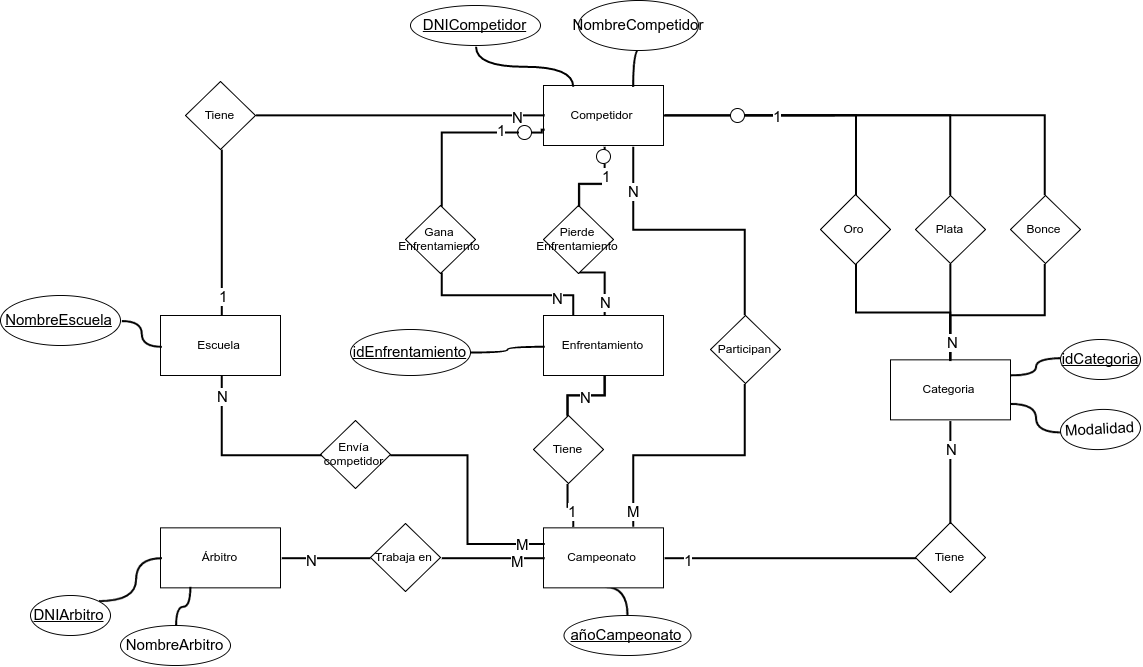
\includegraphics[scale=0.4]{imagenes/DER.png}
  \caption{Diagrama Entidad Relación}
\end{figure}

A continuación detallaremos las distintas entidades y sus relaciones.\\

Los árbitros poseen un DNI, que sirve como identificador y clave primaria, y un nombre. Cada árbitro participo históricamente
en muchos campeonatos.\\

Las escuelas se identifican con un nombre y envían a sus competidores a los distintos campeonatos. Cada escuela conoce los competidores
que posee y los campeonatos a los que mando competidores.\\

Los campeonatos poseen un año, usado como clave primaria. Cada campeonato tiene muchas categorías. Cada una de estas se
traduce en enfrentamientos entre dos competidores. Por lo tanto, el campeonato tiene muchos enfrentamientos. Además
el campeonato registra a los competidores que participan de los enfrentamientos. Como los competidores provienen de
diversas escuelas.\\

Cada categoría es identificada con un idCategoría. Además cada una tiene una modalidad, las cuales pueden ser
Combate, Formas o Rotura. Existen tres tipos de medallas por categoría: oro, plata y bronce. Estas medallas son ganadas
por los competidores de los enfrentamientos de esa categoría.\\

Los competidores tienen como clave primaria su DNI y poseen un nombre. Los competidores representan a una sola escuela en
los campeonatos. A la vez, pueden haber participado en varios campeonatos. Dado que cada competidor puede participar
de varias categorías por campeonato, también puede haber resultado victorioso o derrotado en varios enfrentamientos por
cada campeonato al que participo. También puede haber ganado medallas, de cualquiera de los tres tipo, en más de una categoría.
O podría no haber ganado ninguna.\\

Los enfrentamientos se realizan para un campeonato específico y en él participan dos competidores distintos. Uno de estos
es el ganador del enfrentamiento y otro el perdedor.


\newpage
\section{Modelo de Interacción de Documentos}
En esta sección mostraremos el Diagrama de Interrelación de Documentos (DID) creado a partir del DER mostrado en la sección
anterior.

\begin{figure}[H]
  \centering
    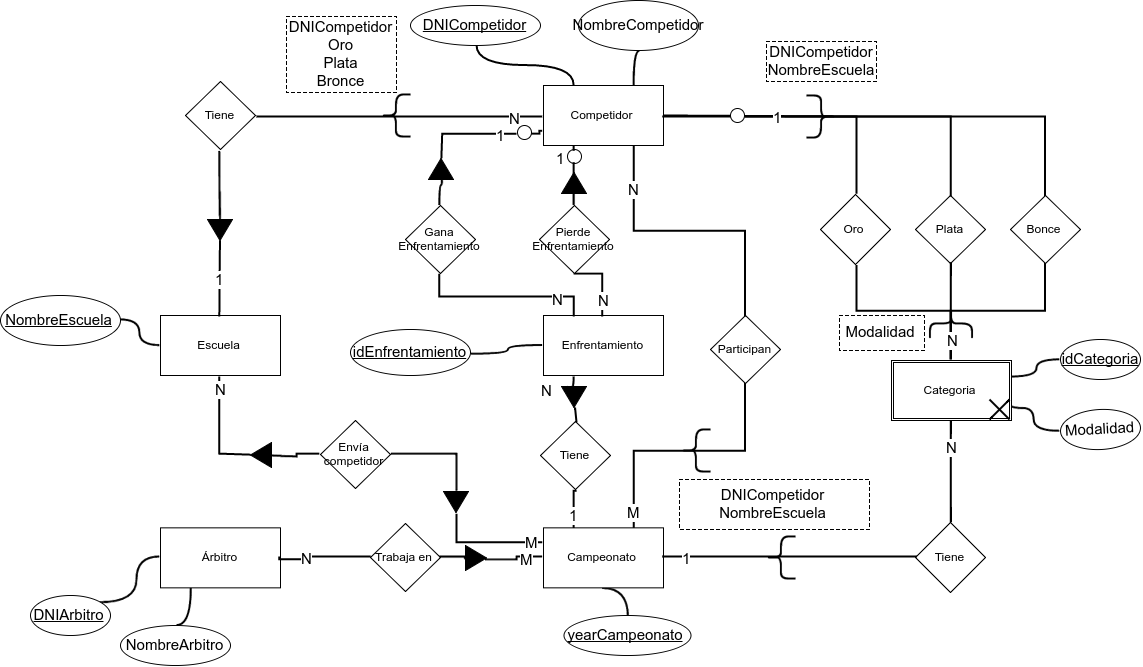
\includegraphics[scale=0.4]{imagenes/DID.png}
  \caption{Diagrama de Interrelación de Documentos}
\end{figure}

A continuación mostraremos la forma en la que se resolvieron las consultas pedidas y justificaremos las decisiones
tomadas para optimizarlas.

\subsection{Consultas}
\begin{enumerate}
  \item Se pide la cantidad de enfrentamientos ganados por competidor para un campeonato dado. Se nos da como parámetro
  el año del campeonato. Para resolver la consulta, recorremos todos los enfrentamientos. Contamos la cantidad de
  enfrentamientos ganados para cada competidor que coincidan con el año del campeonato. Esto lo podemos realizar de forma óptima
  ya que el enfrentamiento referencia a campeonato, por lo tanto tiene su año. Además, referencia al ganador y al
  perdedor, por lo que puede usarlos para contar la cantidad de victorias por cada competidor.

  \item Se pide la cantidad de medallas por nombre de escuela en toda la historia. Iteramos en el documento Escuela y por cada una
  recorremos la ListaCompetidores. Para cada competidor, realizamos la suma de las medallas de los tres tipos (oro, plata y bronce).
  Esta sumatoria se beneficia del hecho de que cada escuela posee la ListaCompetidores gracias a que se tomo la decisión de embeber parcialmente a los competidores en el documento Escuela. La lista de competidores contiene la cantidad de medallas de cada uno de los tres tipos que cada competidor obtuvo
  históricamente. Solo hace falta sumar los tres tipos para obtener el histórico de medallas del competidor.

  \item Para cada escuela, se pide el campeonato donde ganó más medalla. La consulta se divide en dos partes. La primer parte consiste
  en recorrer todos los campeonatos y guardarnos las categorías que están en ListaCategorías, utilizando para esto el año del
  campeonato. En la segunda parte recorremos todas las entradas en el documento Escuela. Por cada una de estas, utilizamos las
  categorías guardadas en el paso anterior. Recorremos todas las categorías y, por cada una, contamos la cantidad de ganadores de
  medallas que pertenecen a la escuela.
  
  Esta consulta está optimizada usando que Campeonato tiene embebido a Categoría, con lo
  cual podemos adquirir de cada campeonato los ganadores de medallas de los tres tipos. Además Categoría tiene embebido parcialmente
  a Competidor por el atributo NombreEscuela, con lo cual podemos usar este dato para identificar a la escuela que pertenece cada
  medalla. Por último, el documento Escuela tiene una referencia a Campeonato. Esto significa que Escuela tiene los yearCampeonato
  de todos en los que mando competidores.
  
  En el primer paso habíamos guardado las categorías por el año del campeonato y,
  gracias a esta referencia de Campeonato en Escuela, podemos acceder a las categorías. Por consiguiente, tenemos acceso a la
  información sobre los ganadores de medallas. Dado que necesitamos la información de las medallas, la consulta pareciera que
  se puede resolver tanto usando el documento Campeonato como el documento Competidor. Sin embargo, esto no es cierto ya que
  a través de competidor no podemos diferenciar los campeonatos en los cuales cada uno gano las medallas. Por eso necesitamos recorrer
  los campeonatos para obtener las categorías y después ver en cuales los competidores de cada escuela resultaron vencedores.

  \item Se pide los árbitros que participaron en al menos 4 campeonatos. La consulta se realiza recorriendo los documentos
  de Árbitro contando los Campeonatos usando ListaCampeonatos. Finalmente nos quedamos con los árbitros donde la ListaCampeonatos
  tiene al menos 4 campeonatos distintos. Para cada árbitro, el proceso se resume en contar los campeonatos en la lista.
  Podemos realizar esto gracias a ListaCampeonatos, la cual obtenemos gracias a que el documento Arbitro posee referencias
  al documento Campeonato.

  \item Se pide las escuelas que han presentado el mayor número de competidores en cada campeonato. Recorremos el conjunto de documentos
  Campeonato y para cada uno recorremos su ListaCompetidores y cuentamos, por cada NombreEscuela, la cantidad de competidores.
  La consulta es optimizada debido a que los Campeonatos tienen embebido parcialmente a Competidor por el atributo
  NombreEscuela. Con lo cual, no se necesita acceder a otro documento que no sean todas las entradas de Campeonatos.
  Esto último es necesario ya que necesitamos información de todos los Campeonatos para encontrar a las escuelas en las
  que más competidores participaron.

  \item Obtener los competidores que más medallas obtuvieron por modalidad. Por cada entrada del documento Campeonato,
  contamos las medallas de cada tipo que coinciden con cada modalidad. Después nos quedamos con el DNICompetidor a los cuales
  son ganadores de más medallas de cada tipo. Esta consulta se beneficia de que el Campeonato tiene embebido
  el documento Categoría. Por lo tanto, no es necesario acceder a ningún otro documento que no sea Campeonato. Desde el embebido
  de Categoría obtenemos los DNI's de los competidores que resultaron ganadores.

\end{enumerate}


\newpage
\section{Diseño lógico}
En esta sección mostraremos el diseño lógico de la base de datos usando \textbf{JSONSchema}.

\begin{lstlisting}
  "Arbitro":{"type": "object",
      "properties": {
          "DNIArbitro": {
              "type": "integer"
          },
          "NombreArbitro": {
              "type": "string"
          },
          "ListaCampeonatos": {"type": "array",
              "items": {
                  "type": "integer"
              }
          }
      }
  }
\end{lstlisting}

\begin{lstlisting}
  "Campeonato":{"type": "object",
      "properties": {
          "yearCampeonato": {
              "type": "integer"
          },
          "ListaCategorias": { "type": "array",
              "items": {"type": "object",
                  "properties": {
                      "GanadorBronce": {
                          "type": "integer"
                      },
                      "GanadorOro": {
                          "type": "integer"
                      },
                      "GanadorPlata": {
                          "type": "integer"
                      },
                      "Modalidad": {
                          "type": "string"
                      },
                      "idCategoria": {
                          "type": "integer"
                      }
                  }

              }
          },
          "ListaCompetidores": {"type": "array",
              "items": { "type": "object",
                  "properties": {
                      "DNICompetidor": {
                          "type": "integer"
                      },
                      "NombreEscuela": {
                          "type": "string"
                      }
                  }
              }
          },
          "ListaEscuelas": {"type": "array",
              "items": {
                  "type": "string"
              }
          }
      }

  }
\end{lstlisting}

\begin{lstlisting}
  "Categoria":{"type": "object",
      "properties": {
          "GanadorBronce": {"type": "object",
              "properties": {
                  "DNICompetidor": {
                      "type": "integer"
                  },
                  "NombreEscuela": {
                      "type": "string"
                  }
              }
          },
          "GanadorOro": {"type": "object",
              "properties": {
                  "DNICompetidor": {
                      "type": "integer"
                  },
                  "NombreEscuela": {
                      "type": "string"
                  }
              }
          },
          "GanadorPlata": {"type": "object",
              "properties": {
                  "DNICompetidor": {
                      "type": "integer"
                  },
                  "NombreEscuela": {
                      "type": "string"
                  }
              }
          },
          "Modalidad": {
              "type": "string"
          },
          "idCategoria": {
              "type": "integer"
          }
      }
  }
\end{lstlisting}

\begin{lstlisting}
  "Competidor":{"type": "object",
      "properties": {
          "Bronce": {"type": "array",
              "items": {
                  "type": "integer"
              }
          },
          "DNICompetidor": {
              "type": "integer"
          },
          "NombreCompetidor": {
              "type": "string"
          },
          "NombreEscuela": {
              "type": "string"
          },
          "Oro": {"type": "array",
              "items": {
                  "type": "integer"
              }
          },
          "Plata": {"type": "array",
              "items": {
                  "type": "integer"
              }
          }
      }
  }
\end{lstlisting}

\begin{lstlisting}
  "Enfrentamiento":{"type": "object",
      "properties": {
          "idEnfrentamiento": {
              "type": "integer"
          },
          "yearCampeonato": {
              "type": "integer"
          }
          "Ganador": {
              "type": "integer"
          }
          "Perdedor": {
              "type": "integer"
          }
      }
  }
\end{lstlisting}

\begin{lstlisting}
  "Escuela":{"type": "object",
      "properties": {
          "ListaCampeonatos": {"type": "array",
              "items": {
                  "type": "integer"
              }
          },
          "ListaCompetidores": {"type": "array",
              "items": {
                  "type": "integer"
              }
          },
          "NombreEscuela": {
              "type": "string"
          }
      }
  }
\end{lstlisting}


\newpage
\section{Conclusiones}
El desarrollo de una base de datos no relacional para guardar el histórico de los Campeonatos Mundiales de
Taekwon-do ITF, consiguió que mostrarnos como funciona en la práctica el diseño e implementación de una base basada en
documentos.\\

El diagrama de entidad relación especifico para el problema resulto ser mucho más fácil de hacer y más corto.
Esto se debe que este diagrama sirve para resolver un problema con menor número de detalles que el visto en el TP1.
Por otro lado, el diagrama de interrelación de documentos resulto en un desafío mucho más interesante. Obligándonos
muchas veces a replantear las decisiones tomadas e, incluso, a modificar el DER. Aunque, en esto último, siempre se hizo
manteniendo la coherencia respecto a las entidades y sus relaciones. Algunas de las dificultades surgidas fueron, por ejemplo,
la representación de categoría o modalidad en un campeonato. Dado que en el trabajo práctico anterior solo se modelaba un
campeonato, las categorías eran exclusivas de este. Sin embargo, al tener muchos campeonatos las categorías se podrían
relacionar con ellos de varias formas. Una de las primeras ideas que se barajaron fue que cada categoría perteneciera a
muchos campeonatos. Al final, para facilitar las consultas se opto por representar cada categoría según el año de cada
campeonato. Con lo cual, hay varias categorías por año sin importar la cantidad que existan en los demás. Las mayoría
de los problemas de diseño fueron solucionados discutiendo como obtener la mejor representación de la base de datos
para optimizar las consultas que se pedían. Se podría concluir que, a pesar de las dificultades de diseño, el modelo de
bases de datos no relacionales basadas en documentos ofrece herramientas que simplifican la implementación, una vez el
diseño está terminado. A su vez, el diseño no presenta grandes dificultades fuera de las decisiones que se deben tomar.
Esto debido a que la notación sobre el DID es clara y fácil de interpretar.


\end{document}
